% 第一章：复数\index{复数}与复平面

\chapter{复数\index{复数}与复平面}

\begin{wulibj}[本章导读]
复数\index{复数}最初是为了解决``负数开方''问题而引入的，后来却发现它在物理学中有广泛的应用：交流电路分析、量子力学波函数、二维势场问题……本章我们将学习复数\index{复数}的基本概念、几何表示和运算，为后续学习复变函数打下基础。
\end{wulibj}

% ========== 第一节 ==========
\section{复数\index{复数}的引入：从解方程到复平面}

\subsection{一个古老的问题}

让我们从一个简单的问题开始：求方程 $x^2 + 1 = 0$ 的解。

在实数范围内，这个方程无解，因为任何实数的平方都是非负的。但是，数学家们想：能不能``发明''一个数，使得它的平方等于 $-1$？

\begin{dingliyi}{}{虚数单位}
引入记号 $\mathrm{i}$（或 $j$），称为\textbf{虚数单位}，规定
\begin{equation}
    \mathrm{i}^2 = -1 \quad \text{或等价地} \quad \mathrm{i} = \sqrt{-1}
\end{equation}
\end{dingliyi}

有了虚数单位，方程 $x^2 + 1 = 0$ 就有解了：$x = \pm \mathrm{i}$。

\subsection{复数\index{复数}的定义}

\begin{dingliyi}{}{复数}
形如
\begin{equation}
    z = x + \mathrm{i}y
\end{equation}
的数称为\textbf{复数\index{复数}}，其中 $x, y$ 是实数，$\mathrm{i}$ 是虚数单位。称 $x$ 为复数\index{复数} $z$ 的\textbf{实部}，记作 $x = \operatorname{Re}(z)$；称 $y$ 为复数\index{复数} $z$ 的\textbf{虚部}，记作 $y = \operatorname{Im}(z)$。

\begin{zhu}{}{}
虚部是 $y$，不是 $\mathrm{i}y$。例如，复数\index{复数} $z = 3 + 2\mathrm{i}$ 的实部是 $3$，虚部是 $2$。
\end{zhu}
\end{dingliyi}

\subsection{复数\index{复数}的分类}

根据实部和虚部的取值，复数\index{复数}可以分为：

\begin{itemize}
    \item \textbf{实数}：虚部为零的复数\index{复数}，即 $y = 0$。
    \item \textbf{纯虚数}：实部为零的复数\index{复数}，即 $x = 0$。
    \item \textbf{虚数}：虚部不为零的复数\index{复数}，即 $y \neq 0$（包括纯虚数和一般的复数\index{复数}）。
\end{itemize}

\begin{lizi}{}{}
    判断以下复数\index{复数}的类型：
    \begin{enumerate}
        \item $z_1 = 5$
        \item $z_2 = 3\mathrm{i}$
        \item $z_3 = 2 + 3\mathrm{i}$
        \item $z_4 = 0$
    \end{enumerate}
    \begin{jie}
        \begin{enumerate}
            \item $z_1 = 5$：实数（虚部为 $0$）
            \item $z_2 = 3\mathrm{i}$：纯虚数（实部为 $0$）
            \item $z_3 = 2 + 3\mathrm{i}$：一般复数\index{复数}
            \item $z_4 = 0$：既是实数又是纯虚数（实部和虚部都为 $0$）
        \end{enumerate}
    \end{jie}
\end{lizi}

\subsection{复平面：几何表示}

复数\index{复数} $z = x + \mathrm{i}y$ 可以用平面上的点 $(x, y)$ 来表示。这个平面称为\textbf{复平面}（或\textbf{阿甘德平面}）。
\begin{figure}[htbp]
\centering
\begin{tikzpicture}[scale=1.2]
    % 坐标轴
    \draw[->, thick] (-0.5, 0) -- (4, 0) node[right] {$x$ (实轴)};
    \draw[->, thick] (0, -0.5) -- (0, 3) node[above] {$y$ (虚轴)};
    
    % 复数\index{复数} z = 3 + 2i
    \coordinate (z) at (3, 2);
    \fill[blue] (z) circle (2pt) node[above right] {$z = 3 + 2\mathrm{i}$};
    
    % 投影
    \draw[dashed, gray] (z) -- (3, 0) node[below] {$3$};
    \draw[dashed, gray] (z) -- (0, 2) node[left] {$2$};
    
    % 向量
    \draw[->, thick, blue!70] (0, 0) -- (z);
    
    % 原点
    \node[below left] at (0, 0) {$O$};
\end{tikzpicture}
\caption{复数\index{复数} $z = 3 + 2\mathrm{i}$ 在复平面上的表示}
\label{fig:complex-plane}
\end{figure}

在复平面中：
\begin{itemize}
    \item \textbf{横轴}称为\textbf{实轴}，表示实部。
    \item \textbf{纵轴}称为\textbf{虚轴}，表示虚部。
    \item 复数\index{复数} $z = x + \mathrm{i}y$ 对应点 $(x, y)$，也可以用从原点到该点的\textbf{向量}表示。
\end{itemize}

\begin{tishi}[几何直观的好处]
把复数\index{复数}表示为平面上的点或向量，可以让我们用几何方法理解复数\index{复数}的运算。后面我们会看到，复数\index{复数}加法就是向量加法，复数\index{复数}乘法对应向量的旋转和伸缩。
\end{tishi}

\subsection{为什么需要复数\index{复数}？}

你可能会问：实数还不够用吗？为什么非要引入复数\index{复数}？

\begin{enumerate}
    \item \textbf{代数完备性}：在复数\index{复数}范围内，任何 $n$ 次多项式方程都有 $n$ 个根（计重数）。这称为\textbf{代数基本定理}。实数没有这个性质。

    \item \textbf{物理应用}：
    \begin{itemize}
        \item \textbf{交流电路}：复数\index{复数}可以简洁地表示交流电的振幅和相位。
        \item \textbf{量子力学}：波函数是复值函数，复数\index{复数}的相位有物理意义。
        \item \textbf{信号处理}：傅里叶变换\index{傅里叶变换}涉及复数\index{复数}，是现代通信的基础。
    \end{itemize}
    
    \item \textbf{数学简化}：很多实数问题用复数\index{复数}处理更简单。例如，计算某些实积分，用复变函数的留数定理\index{留数定理}会出奇地简单。
\end{enumerate}

\begin{tishi}[代数基本定理]
\textbf{定理}：任何 $n$ 次多项式方程
\begin{equation}
    a_n z^n + a_{n-1} z^{n-1} + \cdots + a_1 z + a_0 = 0
\end{equation}
在复数范围内恰好有 $n$ 个根（计重数）。

这是复数相对于实数的根本优势。例如，方程 $x^2 + 1 = 0$ 在实数范围内无解，但在复数范围内有 $z = \pm \mathrm{i}$ 两个根。

\textbf{证明}需要复变函数论的工具（如刘维尔定理），将在第六章给出。
\end{tishi}

\begin{wulibj}[物理背景：交流电路]
在交流电路中，电压和电流都是正弦函数：
\begin{align}
    u(t) &= U_0 \cos(\omega t + \varphi_u) \\
    i(t) &= I_0 \cos(\omega t + \varphi_i)
\end{align}
如果直接用三角函数运算，会非常繁琐。但如果引入复数\index{复数}表示：
\begin{align}
    \tilde{u} &= U_0 \mathrm{e}^{\mathrm{i}\varphi_u} \\
    \tilde{i} &= I_0 \mathrm{e}^{\mathrm{i}\varphi_i}
\end{align}
那么阻抗、功率计算都变成简单的复数\index{复数}运算。
\end{wulibj}

% ========== 第二节 ==========
\section{复数\index{复数}的几何表示：模、辐角、共轭}

\subsection{复数\index{复数}的模}

复数\index{复数} $z = x + \mathrm{i}y$ 的\textbf{模}（或\textbf{绝对值}）定义为
\begin{equation}
    |z| = \sqrt{x^2 + y^2}
\end{equation}

几何上，模 $|z|$ 表示从原点到点 $z$ 的距离，也就是向量的长度。

\begin{figure}[htbp]
\centering
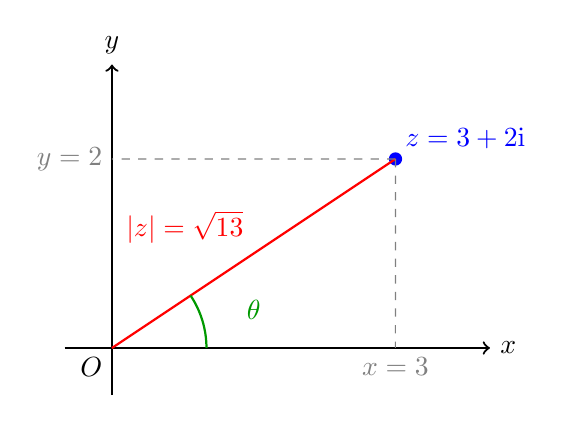
\begin{tikzpicture}[scale=1.2]
    % 坐标轴
    \draw[->, thick] (-0.5, 0) -- (4, 0) node[right] {$x$};
    \draw[->, thick] (0, -0.5) -- (0, 3) node[above] {$y$};
    
    % 复数\index{复数} z = 3 + 2i
    \coordinate (z) at (3, 2);
    \fill[blue] (z) circle (2pt) node[above right] {$z = 3 + 2\mathrm{i}$};
    
    % 模
    \draw[thick, red] (0, 0) -- (z) node[midway, above left] {$|z| = \sqrt{13}$};
    
    % 辐角
    \draw[thick, green!60!black] (1, 0) arc (0:33.69:1);
    \node[green!60!black] at (1.5, 0.4) {$\theta$};
    
    % 坐标分量
    \draw[dashed, gray] (z) -- (3, 0) node[below] {$x=3$};
    \draw[dashed, gray] (z) -- (0, 2) node[left] {$y=2$};
    
    \node[below left] at (0, 0) {$O$};
\end{tikzpicture}
\caption{复数\index{复数}的模与辐角}
\label{fig:modulus-argument}
\end{figure}

\begin{lizi}{}{}
计算复数\index{复数} $z = 3 + 2\mathrm{i}$ 的模。
\begin{jie}
    $|z| = \sqrt{3^2 + 2^2} = \sqrt{9 + 4} = \sqrt{13}$
\end{jie}
\end{lizi}

\subsection{复数\index{复数}的辐角}

复数\index{复数} $z \neq 0$ 的\textbf{辐角} $\theta$ 是实轴正方向到向量 $\overrightarrow{Oz}$ 的夹角：
\begin{equation}
    \tan\theta = \frac{y}{x}
\end{equation}
辐角有无穷多个值，相差 $2\pi$ 的整数倍。满足 $-\pi < \theta \leq \pi$ 的辐角称为\textbf{主辐角}，记作 $\operatorname{Arg}(z)$，而全体辐角记作 $\arg(z) = \operatorname{Arg}(z) + 2k\pi$（$k \in \mathbb{Z}$）。

\begin{jinshi}[常见错误：直接用反正切]
计算辐角时，不能简单地用 $\theta = \arctan(y/x)$，因为反正切函数的值域是 $(-\pi/2, \pi/2)$，无法区分第二、三象限的点。

正确的做法是：
\begin{itemize}
    \item 先根据 $x, y$ 的符号确定象限。
    \item 再用 $\arctan$ 计算参考角。
\end{itemize}
\end{jinshi}

\begin{lizi}{}{}
求复数\index{复数} $z = -1 - \mathrm{i}$ 的模和主辐角。
\begin{jie}
    模：$|z| = \sqrt{(-1)^2 + (-1)^2} = \sqrt{2}$

    主辐角：点 $(-1, -1)$ 在第三象限。$\arctan(1) = \pi/4$，所以主辐角为 $-\pi + \pi/4 = -3\pi/4$。
\end{jie}
\end{lizi}

\subsection{复数\index{复数}的三角形式与指数形式}

利用模和辐角，复数\index{复数}可以表示为\textbf{三角形式}：
\begin{equation}
    z = |z|(\cos\theta + \mathrm{i}\sin\theta) = r(\cos\theta + \mathrm{i}\sin\theta)
\end{equation}
其中 $r = |z|$，$\theta$ 是辐角。

利用\keyword{欧拉公式}（下一章证明）：
\begin{zhongyao}[欧拉公式]
    $\mathrm{e}^{\mathrm{i}\theta} = \cos\theta + \mathrm{i}\sin\theta$
\end{zhongyao}
复数\index{复数}还可以写成\textbf{指数形式}（或\textbf{极坐标形式}）：
\begin{equation}
    z = r\mathrm{e}^{\mathrm{i}\theta}
\end{equation}

\begin{tishi}[三种形式的选择]
\begin{itemize}
    \item \textbf{代数形式} $z = x + \mathrm{i}y$：适合加法、减法。
    \item \textbf{三角形式} $z = r(\cos\theta + \mathrm{i}\sin\theta)$：适合推导公式。
    \item \textbf{指数形式} $z = r\mathrm{e}^{\mathrm{i}\theta}$：适合乘法、除法、幂运算。
\end{itemize}
解题时根据运算类型选择合适的形式。
\end{tishi}

\subsection{共轭复数\index{复数}}

复数\index{复数} $z = x + \mathrm{i}y$ 的\textbf{共轭复数\index{复数}}定义为
\begin{equation}
    \bar{z} = x - \mathrm{i}y
\end{equation}
即把虚部取相反数。

几何上，共轭复数\index{复数} $\bar{z}$ 关于实轴与 $z$ 对称。

\begin{figure}[htbp]
\centering
\begin{tikzpicture}[scale=1.2]
    % 坐标轴
    \draw[->, thick] (-0.5, 0) -- (4, 0) node[right] {$x$};
    \draw[->, thick] (0, -2.5) -- (0, 2.5) node[above] {$y$};
    
    % 复数\index{复数} z
    \coordinate (z) at (3, 2);
    \fill[blue] (z) circle (2pt) node[above right] {$z = 3 + 2\mathrm{i}$};
    
    % 共轭复数\index{复数}
    \coordinate (zbar) at (3, -2);
    \fill[red] (zbar) circle (2pt) node[below right] {$\bar{z} = 3 - 2\mathrm{i}$};
    
    % 对称线
    \draw[dashed, gray] (z) -- (zbar);
    
    \node[below left] at (0, 0) {$O$};
\end{tikzpicture}
\caption{共轭复数\index{复数}的几何意义}
\label{fig:conjugate}
\end{figure}

共轭复数\index{复数}有以下重要性质：

\begin{dingli}{}{共轭复数的性质}
设 $z = x + \mathrm{i}y$，则：
\begin{enumerate}
    \item $z + \bar{z} = 2x = 2\operatorname{Re}(z)$
    \item $z - \bar{z} = 2\mathrm{i}y = 2\mathrm{i}\operatorname{Im}(z)$
    \item $z\bar{z} = |z|^2 = x^2 + y^2$
    \item $\overline{z_1 + z_2} = \bar{z}_1 + \bar{z}_2$
    \item $\overline{z_1 z_2} = \bar{z}_1 \bar{z}_2$
    \item $\overline{z^n} = (\bar{z})^n$
    \item $|\bar{z}| = |z|$
    \item $\arg(\bar{z}) = -\arg(z)$
\end{enumerate}
\end{dingli}

\begin{proof}
我们证明第3条性质，其余留给读者。

设 $z = x + \mathrm{i}y$，则 $\bar{z} = x - \mathrm{i}y$。
\begin{align}
    z\bar{z} &= (x + \mathrm{i}y)(x - \mathrm{i}y) \\
             &= x^2 - \mathrm{i}xy + \mathrm{i}xy - \mathrm{i}^2 y^2 \\
             &= x^2 + y^2 = |z|^2
\end{align}
\end{proof}

\begin{lizi}{}{}
利用共轭复数\index{复数}计算 $\displaystyle\frac{3 + 2\mathrm{i}}{1 - \mathrm{i}}$。
\begin{jie}
    将分母``实数化''：分子分母同乘分母的共轭复数\index{复数}。
    \begin{align}
        \frac{3 + 2\mathrm{i}}{1 - \mathrm{i}} &= \frac{(3 + 2\mathrm{i})(1 + \mathrm{i})}{(1 - \mathrm{i})(1 + \mathrm{i})} \\
        &= \frac{3 + 3\mathrm{i} + 2\mathrm{i} + 2\mathrm{i}^2}{1 - \mathrm{i}^2} \\
        &= \frac{3 + 5\mathrm{i} - 2}{2} \\
        &= \frac{1 + 5\mathrm{i}}{2} = \frac{1}{2} + \frac{5}{2}\mathrm{i}
    \end{align}
\end{jie}
\end{lizi}

% ========== 第三节 ==========
\section{复数\index{复数}的运算与几何意义}

\subsection{加法与减法}

\begin{dingliyi}{}{复数的加减}
设 $z_1 = x_1 + \mathrm{i}y_1$，$z_2 = x_2 + \mathrm{i}y_2$，则
\begin{align}
    z_1 + z_2 &= (x_1 + x_2) + \mathrm{i}(y_1 + y_2) \\
    z_1 - z_2 &= (x_1 - x_2) + \mathrm{i}(y_1 - y_2)
\end{align}
\end{dingliyi}

\textbf{几何意义}：复数\index{复数}加法对应向量加法（平行四边形法则或三角形法则），减法对应向量减法。

\begin{figure}[htbp]
\centering
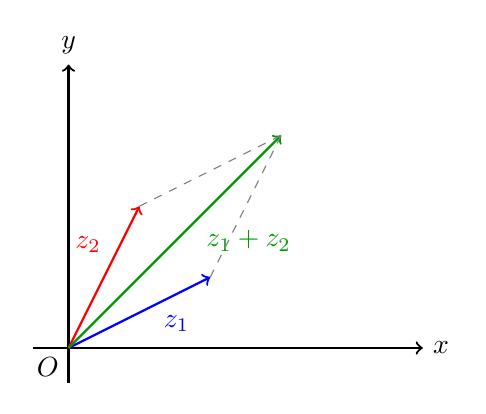
\begin{tikzpicture}[scale=0.9]
    % 坐标轴
    \draw[->, thick] (-0.5, 0) -- (5, 0) node[right] {$x$};
    \draw[->, thick] (0, -0.5) -- (0, 4) node[above] {$y$};
    
    % 向量 z1, z2
    \coordinate (z1) at (2, 1);
    \coordinate (z2) at (1, 2);
    \coordinate (zsum) at (3, 3);
    
    \draw[->, thick, blue] (0, 0) -- (z1) node[pos=0.6, below right] {$z_1$};
    \draw[->, thick, red] (0, 0) -- (z2) node[pos=0.6, above left] {$z_2$};
    \draw[->, thick, green!60!black] (0, 0) -- (zsum) node[pos=0.6, below right] {$z_1+z_2$};
    
    % 平行四边形
    \draw[dashed, gray] (z1) -- (zsum);
    \draw[dashed, gray] (z2) -- (zsum);
    
    \node[below left] at (0, 0) {$O$};
\end{tikzpicture}
\caption{复数\index{复数}加法的平行四边形法则}
\label{fig:complex-add}
\end{figure}

\subsection{乘法}

\begin{dingliyi}{}{复数的乘法}
设 $z_1 = x_1 + \mathrm{i}y_1$，$z_2 = x_2 + \mathrm{i}y_2$，则
\begin{equation}
    z_1 z_2 = (x_1 x_2 - y_1 y_2) + \mathrm{i}(x_1 y_2 + x_2 y_1)
\end{equation}
\end{dingliyi}

这个公式不太好记。如果用指数形式，就简单多了：

设 $z_1 = r_1 \mathrm{e}^{\mathrm{i}\theta_1}$，$z_2 = r_2 \mathrm{e}^{\mathrm{i}\theta_2}$，则
\begin{equation}
    z_1 z_2 = r_1 r_2 \mathrm{e}^{\mathrm{i}(\theta_1 + \theta_2)}
\end{equation}

\textbf{几何意义}：两个复数相乘，模相乘，辐角相加。这意味着：
\begin{itemize}
    \item \keyword{模}乘以 $r_2$：向量的长度伸缩 $r_2$ 倍。
    \item \keyword{辐角}加 $\theta_2$：向量逆时针旋转 $\theta_2$ 角。
\end{itemize}

\begin{figure}[htbp]
\centering
\begin{tikzpicture}[scale=0.85]
    % z 平面
    \begin{scope}
        \draw[->, thick, gray] (-0.5, 0) -- (4.5, 0) node[right] {$x$};
        \draw[->, thick, gray] (0, -0.5) -- (0, 3.5) node[above] {$y$};
        
        % z1
        \coordinate (z1) at (2, 1);
        \draw[->, very thick, blue] (0, 0) -- (z1);
        \fill[blue] (z1) circle (2pt) node[above right] {$z_1$};
        \draw[blue, dashed] (0, 0) -- (2, 0) node[below] {$r_1$};
        \draw[blue, thick] (0.6, 0) arc (0:26.57:0.6);
        \node[blue] at (0.9, 0.25) {$\theta_1$};
        
        % z2
        \coordinate (z2) at (1, 2.5);
        \draw[->, very thick, red] (0, 0) -- (z2);
        \fill[red] (z2) circle (2pt) node[above] {$z_2$};
        \draw[red, thick] (0.4, 0) arc (0:68.2:0.4);
        \node[red] at (0.5, 0.6) {$\theta_2$};
        
        \node at (2, -1) {$z$ 平面};
    \end{scope}
    
    % 箭头
    \draw[->, very thick, purple!70!black] (5, 1.5) -- (6.5, 1.5) node[midway, above] {$\times z_2$};
    
    % w 平面
    \begin{scope}[xshift=8cm]
        \draw[->, thick, gray] (-0.5, 0) -- (5, 0) node[right] {$x$};
        \draw[->, thick, gray] (0, -0.5) -- (0, 4.5) node[above] {$y$};
        
        % z1*z2 (模变大，角度增加)
        \coordinate (prod) at (2.5, 4);
        \draw[->, very thick, purple!70!black] (0, 0) -- (prod);
        \fill[purple!70!black] (prod) circle (2pt) node[above right] {$z_1 z_2$};
        
        % 原来的z1（虚线）
        \draw[dashed, blue!50] (0, 0) -- (2, 1);
        
        % 模标注
        \draw[purple!70!black, dashed] (0, 0) -- (2.5, 0) node[below] {$r_1 r_2$};
        \draw[purple!70!black, thick] (0.8, 0) arc (0:58:0.8);
        \node[purple!70!black] at (1.3, 0.7) {$\theta_1+\theta_2$};
        
        \node at (2.5, -1) {$w$ 平面};
    \end{scope}
\end{tikzpicture}
\caption{复数乘法的几何意义：模伸缩、辐角相加}
\label{fig:complex-mult}
\end{figure}

\begin{tishi}[乘以 $\mathrm{i}$ 的几何意义]
$\mathrm{i} = \mathrm{e}^{\mathrm{i}\pi/2}$，模为 $1$，辐角为 $\pi/2$（即 $90°$）。因此，任何复数 $z$ 乘以 $\mathrm{i}$，相当于：
\begin{itemize}
    \item 模不变（$|\mathrm{i}| = 1$）
    \item 辐角增加 $90°$，即逆时针旋转 $90°$
\end{itemize}
这正是为什么 $\mathrm{i}$ 在交流电路中代表 $90°$ 相位差的原因。
\end{tishi}

\begin{wulibj}[复数乘法与旋转矩阵]
复数乘法与二维旋转矩阵有深刻的对应关系。

设 $z_2 = \cos\theta + \mathrm{i}\sin\theta$（模为 $1$ 的复数），则 $z_1 \cdot z_2$ 相当于把 $z_1$ 旋转 $\theta$ 角。

用代数形式展开：设 $z_1 = x + \mathrm{i}y$，$z_2 = \cos\theta + \mathrm{i}\sin\theta$，则
\begin{align}
    z_1 z_2 &= (x + \mathrm{i}y)(\cos\theta + \mathrm{i}\sin\theta) \notag \\
           &= (x\cos\theta - y\sin\theta) + \mathrm{i}(x\sin\theta + y\cos\theta)
\end{align}
这与二维旋转矩阵的作用完全一致：
\begin{equation}
    \begin{pmatrix} x' \\ y' \end{pmatrix} = 
    \begin{pmatrix} \cos\theta & -\sin\theta \\ \sin\theta & \cos\theta \end{pmatrix}
    \begin{pmatrix} x \\ y \end{pmatrix}
\end{equation}
也就是说：\textbf{复数乘法等价于二维平面上的旋转变换}（当模为 $1$ 时）或旋转加缩放变换（一般情况）。这个对应关系在计算机图形学、机器人学中有广泛应用。
\end{wulibj}

\begin{lizi}{}{}
设 $z = 1 + \mathrm{i}$，求 $z^4$。
\begin{jie}
    先化成指数形式。$|z| = \sqrt{2}$，$\theta = \pi/4$，所以
    \begin{equation}
        z = \sqrt{2}\,\mathrm{e}^{\mathrm{i}\pi/4}
    \end{equation}
    于是
    \begin{equation}
        z^4 = (\sqrt{2})^4 \mathrm{e}^{\mathrm{i}\pi} = 4(-1) = -4
    \end{equation}
\end{jie}
\end{lizi}

\subsection{除法}

\begin{dingliyi}{}{复数的除法}
设 $z_1 = x_1 + \mathrm{i}y_1$，$z_2 = x_2 + \mathrm{i}y_2 \neq 0$，则
\begin{equation}
    \frac{z_1}{z_2} = \frac{z_1 \bar{z}_2}{|z_2|^2} = \frac{(x_1 x_2 + y_1 y_2) + \mathrm{i}(x_2 y_1 - x_1 y_2)}{x_2^2 + y_2^2}
\end{equation}
\end{dingliyi}

用指数形式更简洁：若 $z_1 = r_1 \mathrm{e}^{\mathrm{i}\theta_1}$，$z_2 = r_2 \mathrm{e}^{\mathrm{i}\theta_2}$，则
\begin{equation}
    \frac{z_1}{z_2} = \frac{r_1}{r_2} \mathrm{e}^{\mathrm{i}(\theta_1 - \theta_2)}
\end{equation}

\textbf{几何意义}：模相除，辐角相减。

\subsection{乘方与开方}

\subsubsection{乘方}

设 $z = r\mathrm{e}^{\mathrm{i}\theta}$，则 $z$ 的 $n$ 次幂为
\begin{equation}
    z^n = r^n \mathrm{e}^{\mathrm{i}n\theta}
\end{equation}

特别地，当 $r = 1$ 时，有\textbf{棣莫弗公式}：
\begin{equation}
    (\cos\theta + \mathrm{i}\sin\theta)^n = \cos n\theta + \mathrm{i}\sin n\theta
\end{equation}
\begin{lizi}{}{}
用棣莫弗公式计算 $\cos 3\theta$。
\begin{jie}
    由棣莫弗公式：
    \begin{align}
        \cos 3\theta + \mathrm{i}\sin 3\theta &= (\cos\theta + \mathrm{i}\sin\theta)^3 \\
        &= \cos^3\theta + 3\mathrm{i}\cos^2\theta\sin\theta - 3\cos\theta\sin^2\theta - \mathrm{i}\sin^3\theta
    \end{align}
    比较实部，得
    \begin{equation}
        \cos 3\theta = \cos^3\theta - 3\cos\theta\sin^2\theta = 4\cos^3\theta - 3\cos\theta
    \end{equation}
\end{jie}
\end{lizi}

\subsubsection{开方}

设 $z = r\mathrm{e}^{\mathrm{i}\theta}$，求 $z$ 的 $n$ 次方根 $w = \sqrt[n]{z}$。

设 $w = \rho\mathrm{e}^{\mathrm{i}\varphi}$，则 $w^n = z$ 给出
\begin{equation}
    \rho^n \mathrm{e}^{\mathrm{i}n\varphi} = r\mathrm{e}^{\mathrm{i}\theta}
\end{equation}
因此 $\rho = \sqrt[n]{r}$，$n\varphi = \theta + 2k\pi$（$k = 0, 1, \ldots, n-1$），即
\begin{equation}
    \varphi_k = \frac{\theta + 2k\pi}{n}, \quad k = 0, 1, \ldots, n-1
\end{equation}

所以 $z$ 的 $n$ 次方根有 $n$ 个值：
\begin{equation}
    w_k = \sqrt[n]{r} \, \mathrm{e}^{\mathrm{i}(\theta + 2k\pi)/n}, \quad k = 0, 1, \ldots, n-1
\end{equation}

\begin{tishi}[几何意义]
$n$ 次方根的 $n$ 个值均匀分布在以原点为圆心、$\sqrt[n]{|z|}$ 为半径的圆周上，构成一个正 $n$ 边形。
\end{tishi}

\begin{figure}[htbp]
\centering
\begin{tikzpicture}[scale=1.5]
    % 圆
    \draw[gray, dashed] (0,0) circle (1);
    
    % 坐标轴
    \draw[->, thick] (-1.5, 0) -- (1.5, 0) node[right] {$x$};
    \draw[->, thick] (0, -1.5) -- (0, 1.5) node[above] {$y$};
    
    % 单位根
    \foreach \k in {0,1,2,3,4,5} {
        \pgfmathsetmacro{\angle}{60*\k}
        \coordinate (w\k) at (\angle:1);
        \fill[blue] (w\k) circle (1.5pt);
        \node at (\angle:1.25) {$w_{\k}$};
    }
    
    % 连接成正六边形
    \draw[blue!50, thick] (w0) -- (w1) -- (w2) -- (w3) -- (w4) -- (w5) -- cycle;
    
    \node[below] at (0, -1.8) {$1$ 的 $6$ 次方根};
\end{tikzpicture}
\caption{$1$ 的 $n$ 次方根构成正 $n$ 边形}
\label{fig:roots-unity}
\end{figure}

\begin{lizi}{}{}
求 $z = 1$ 的立方根。
\begin{jie}
    写成指数形式：$z = 1 = \mathrm{e}^{\mathrm{i}\cdot 0}$。
    
    立方根为
    \begin{equation}
        w_k = \mathrm{e}^{\mathrm{i} \cdot 2k\pi/3}, \quad k = 0, 1, 2
    \end{equation}
    
    即
    \begin{align}
        w_0 &= \mathrm{e}^0 = 1 \\
        w_1 &= \mathrm{e}^{\mathrm{i}2\pi/3} = -\frac{1}{2} + \frac{\sqrt{3}}{2}\mathrm{i} \\
        w_2 &= \mathrm{e}^{\mathrm{i}4\pi/3} = -\frac{1}{2} - \frac{\sqrt{3}}{2}\mathrm{i}
    \end{align}
    
    这三个值在复平面上构成正三角形。
\end{jie}
\end{lizi}

% ========== 第四节 ==========
\section{复平面上的点集：区域、曲线、连通性}

在研究复变函数之前，我们需要先了解复平面上的一些基本概念。这些概念是后续讨论函数定义域、积分路径等的基础。

\subsection{点的邻域}

\begin{dingliyi}{}{邻域}
设 $z_0$ 是复平面上的一个点，$\varepsilon > 0$ 是正数。点集
\begin{equation}
    U(z_0, \varepsilon) = \{z \in \mathbb{C} : |z - z_0| < \varepsilon\}
\end{equation}
称为点 $z_0$ 的\textbf{$\varepsilon$ 邻域}，即以 $z_0$ 为圆心、$\varepsilon$ 为半径的开圆盘。
\end{dingliyi}

\begin{figure}[htbp]
\centering
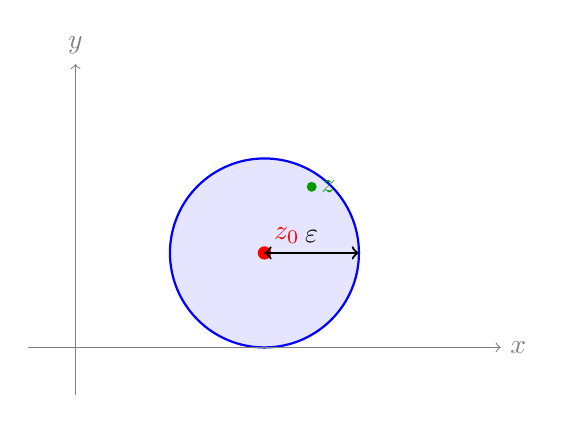
\begin{tikzpicture}[scale=1.2]
    % 圆
    \draw[blue, thick, fill=blue!10] (2, 1) circle (1);
    
    % 圆心
    \fill[red] (2, 1) circle (2pt) node[above right] {$z_0$};
    
    % 半径
    \draw[<->, thick] (2, 1) -- (3, 1) node[midway, above] {$\varepsilon$};
    
    % 任意点
    \fill[green!60!black] (2.5, 1.7) circle (1.5pt) node[right] {$z$};
    
    % 坐标轴
    \draw[->, gray] (-0.5, 0) -- (4.5, 0) node[right] {$x$};
    \draw[->, gray] (0, -0.5) -- (0, 3) node[above] {$y$};
\end{tikzpicture}
\caption{点 $z_0$ 的 $\varepsilon$ 邻域}
\label{fig:neighborhood}
\end{figure}

\subsection{内点、外点、边界点}

\begin{dingliyi}{}{内点、外点、边界点}
设 $E$ 是复平面上的一个点集，$z_0$ 是一个点。
\begin{itemize}
    \item 若存在 $\varepsilon > 0$，使得 $U(z_0, \varepsilon) \subset E$，则称 $z_0$ 是 $E$ 的\textbf{内点}。
    \item 若存在 $\varepsilon > 0$，使得 $U(z_0, \varepsilon) \cap E = \emptyset$，则称 $z_0$ 是 $E$ 的\textbf{外点}。
    \item 若 $z_0$ 既不是 $E$ 的内点也不是外点，即 $z_0$ 的任意邻域内既有 $E$ 中的点又有不在 $E$ 中的点，则称 $z_0$ 是 $E$ 的\textbf{边界点}。
\end{itemize}
\end{dingliyi}

\begin{lizi}{}{}
    设 $E = \{z : |z| < 1\}$ 是单位开圆盘。判断以下点的类型：
    \begin{enumerate}
        \item $z_1 = 0$
        \item $z_2 = 1$
        \item $z_3 = 2$
    \end{enumerate}
    \begin{jie}
        \begin{enumerate}
            \item $z_1 = 0$：内点。因为存在邻域 $U(0, 0.5) \subset E$，完全在 $E$ 内。
            \item $z_2 = 1$：边界点。任意邻域 $U(1, \varepsilon)$ 内既有 $E$ 中的点（如 $1 - \varepsilon/2$），又有 $E$ 外的点（如 $1 + \varepsilon/2$）。
            \item $z_3 = 2$：外点。存在邻域 $U(2, 0.5)$ 与 $E$ 不相交。
        \end{enumerate}
    \end{jie}
\end{lizi}

\subsection{开集与闭集}

\begin{dingliyi}{}{开集与闭集}
\begin{itemize}
    \item 若点集 $E$ 中的每个点都是内点，则称 $E$ 是\textbf{开集}。
    \item 若点集 $E$ 的补集 $\mathbb{C} \setminus E$ 是开集，则称 $E$ 是\textbf{闭集}。
    \item 点集 $E$ 的所有边界点构成的集合称为 $E$ 的\textbf{边界}，记作 $\partial E$。
\end{itemize}
\end{dingliyi}

\begin{zhu}{}{}
``开''和``闭''不是互斥的。例如，空集 $\emptyset$ 和全空间 $\mathbb{C}$ 既开又闭。
\end{zhu}

\subsection{区域}

\begin{dingliyi}{}{区域}
若点集 $D$ 满足：
\begin{enumerate}
    \item $D$ 是开集；
    \item $D$ 是连通的，即 $D$ 中任意两点都可以用一条完全在 $D$ 内的曲线连接。
\end{enumerate}
则称 $D$ 是一个\textbf{区域}。

区域 $D$ 连同它的边界 $\partial D$ 构成的集合称为\textbf{闭区域}，记作 $\bar{D} = D \cup \partial D$。
\end{dingliyi}

\begin{figure}[htbp]
\centering
\begin{tikzpicture}[scale=0.8]
    % 左图：区域
    \begin{scope}
        \draw[blue, thick, fill=blue!20] (0, 0) circle (1.5);
        \draw[blue, thick, fill=blue!20] (2.5, 0) circle (1);
        % 连接部分
        \draw[blue, thick, fill=blue!20] (0, 0) -- (2.5, 0);
        
        \node at (1.25, -2.5) {(a) 区域（连通开集）};
    \end{scope}
    
    % 右图：非区域
    \begin{scope}[xshift=7cm]
        \draw[blue, thick, fill=blue!20] (0, 0) circle (1.5);
        \draw[blue, thick, fill=blue!20] (3, 0) circle (1);
        % 不连接
        
        \node at (1.5, -2.5) {(b) 非区域（不连通）};
    \end{scope}
\end{tikzpicture}
\caption{区域与非区域的区别}
\label{fig:region}
\end{figure}

\subsection{单连通与多连通区域}

\begin{dingliyi}{}{单连通区域}
若区域 $D$ 内任意一条简单闭曲线的内部仍在 $D$ 内，则称 $D$ 是\textbf{单连通区域}。否则称为\textbf{多连通区域}。

直观地说，单连通区域是``没有洞''的区域。
\end{dingliyi}

\begin{figure}[htbp]
\centering
\begin{tikzpicture}[scale=0.9]
    % 单连通
    \begin{scope}
        \draw[blue, thick, fill=blue!20] (0, 0) ellipse (1.5 and 1);
        \node at (0, -2) {(a) 单连通区域};
        
        % 闭曲线
        \draw[red, thick, dashed] (0, 0) circle (0.5);
        \node[red] at (0, 0.8) {\small 闭曲线};
    \end{scope}
    
    % 多连通
    \begin{scope}[xshift=5cm]
        \draw[blue, thick, fill=blue!20] (0, 0) ellipse (1.5 and 1);
        \draw[white, thick, fill=white] (0, 0) circle (0.4);
        \draw[blue, thick] (0, 0) circle (0.4);
        \node at (0, -2) {(b) 多连通区域（有洞）};
        
        % 闭曲线
        \draw[red, thick, dashed] (0, 0) circle (0.25);
    \end{scope}
    
    % 环形区域
    \begin{scope}[xshift=10cm]
        \draw[blue, thick, fill=blue!20] (0, 0) circle (1.5);
        \draw[white, thick, fill=white] (0, 0) circle (0.5);
        \draw[blue, thick] (0, 0) circle (0.5);
        \node at (0, -2) {(c) 环形区域（多连通）};
    \end{scope}
\end{tikzpicture}
\caption{单连通与多连通区域}
\label{fig:simply-connected}
\end{figure}

\begin{zhu}{}{}
单连通与多连通的区别在研究柯西积分定理\index{柯西积分定理}时非常重要。简单来说：
\begin{itemize}
    \item 在单连通区域内，闭路积分可以``收缩''为一点。
    \item 在多连通区域内，围绕``洞''的闭路积分可能不为零。
\end{itemize}
\end{zhu}

% ========== 第五节 ==========
\section{复球面与扩充复平面}

到目前为止，我们用平面上的点来表示复数。但当我们讨论无穷远点时，平面表示会遇到困难——无穷远点在哪里？为了解决这个问题，我们引入复球面（黎曼球面）的概念。

\subsection{球极投影}

考虑一个单位球面，放在复平面上方，使得球的南极与原点相切。设球的北极为 $N$，南极为 $S$。

\begin{dingliyi}{}{球极投影}
对于复平面上任意一点 $z$，连接 $N$ 和 $z$ 的直线与球面相交于一点 $P$（异于 $N$）。这个映射 $z \mapsto P$ 称为\textbf{球极投影}。
\end{dingliyi}

\begin{figure}[htbp]
\centering
\begin{tikzpicture}[scale=1.0]
    % 球面
    \shade[ball color=blue!20, opacity=0.6] (0, 0) circle (1.5);
    \draw[thick] (0, 0) circle (1.5);
    
    % 坐标轴（复平面）
    \draw[->, thick] (-3, -1.5) -- (3, -1.5) node[right] {$x$};
    \draw[->, thick] (0, -1.5) -- (0, 2.5) node[above] {$y$};
    
    % 复平面上的点
    \coordinate (z) at (2, -1.5);
    \fill[red] (z) circle (2pt) node[below] {$z$};
    
    % 北极
    \coordinate (N) at (0, 1.5);
    \fill[blue] (N) circle (2pt) node[above right] {$N$};
    
    % 南极
    \coordinate (S) at (0, -1.5);
    \fill[green!60!black] (S) circle (2pt) node[below] {$S$ (原点)};
    
    % 球面上的点 P
    \coordinate (P) at (1.2, 0.6);
    \fill[orange] (P) circle (2pt) node[right] {$P$};
    
    % 投影线
    \draw[dashed, thick, purple] (N) -- (z);
    
    % 标注
    \node at (0, -2.5) {复平面};
    \node at (2.2, 2) {球面};
\end{tikzpicture}
\caption{球极投影：复平面上的点 $z$ 映射到球面上的点 $P$}
\label{fig:stereographic}
\end{figure}

通过球极投影，复平面上的每一点都唯一对应球面上的一个点（除北极 $N$ 外）。

\subsection{无穷远点}

当复平面上的点 $z$ 越来越远离原点（即 $|z| \to \infty$）时，投影点 $P$ 会越来越接近北极 $N$。

\begin{dingliyi}{}{无穷远点}
在球极投影下，北极 $N$ 对应复平面上的一个特殊的点，称为\textbf{无穷远点}，记作 $\infty$。
\end{dingliyi}

引入无穷远点后，复平面被扩充为\textbf{扩充复平面}（或\textbf{闭复平面}）：
\begin{equation}
    \overline{\mathbb{C}} = \mathbb{C} \cup \{\infty\}
\end{equation}

\begin{tishi}[无穷远点的直观理解]
无穷远点 $\infty$ 可以理解为：
\begin{itemize}
    \item 模 $|z|$ 趋于无穷大的点的极限位置
    \item 不论从哪个方向趋向无穷，最终都到达同一个点 $\infty$
    \item 在复球面上，$\infty$ 就是北极 $N$
\end{itemize}
这与实数中的 $+\infty$ 和 $-\infty$ 不同——复平面中只有一个无穷远点。
\end{tishi}

\subsection{无穷远点的运算}

对于无穷远点，我们可以定义一些合理的运算：

\begin{dingliyi}{}{无穷远点的运算规则}
设 $z \in \mathbb{C}$ 是有限复数，$z \neq 0$。约定：
\begin{align}
    z + \infty &= \infty + z = \infty \\
    z \cdot \infty &= \infty \cdot z = \infty \quad (z \neq 0) \\
    \frac{z}{0} &= \infty \quad (z \neq 0) \\
    \frac{z}{\infty} &= 0 \\
    \frac{\infty}{z} &= \infty \quad (z \neq 0)
\end{align}
\end{dingliyi}

\begin{jinshi}[无定义的运算]
以下运算在扩充复平面中仍然无定义：
\begin{itemize}
    \item $\infty + \infty$
    \item $\infty - \infty$
    \item $\infty \cdot 0$ 和 $0 \cdot \infty$
    \item $\frac{\infty}{\infty}$
    \item $\frac{0}{0}$
\end{itemize}
这些都是不定式，需要具体情况具体分析。
\end{jinshi}

\subsection{扩充复平面的拓扑}

在扩充复平面 $\overline{\mathbb{C}}$ 上，无穷远点 $\infty$ 也有它的邻域：

\begin{dingliyi}{}{无穷远点的邻域}
点集
\begin{equation}
    U(\infty, R) = \{z \in \mathbb{C} : |z| > R\} \cup \{\infty\}
\end{equation}
称为无穷远点的\textbf{$R$ 邻域}，即复平面上圆 $|z| = R$ 外部的区域加上 $\infty$。
\end{dingliyi}

\begin{figure}[htbp]
\centering
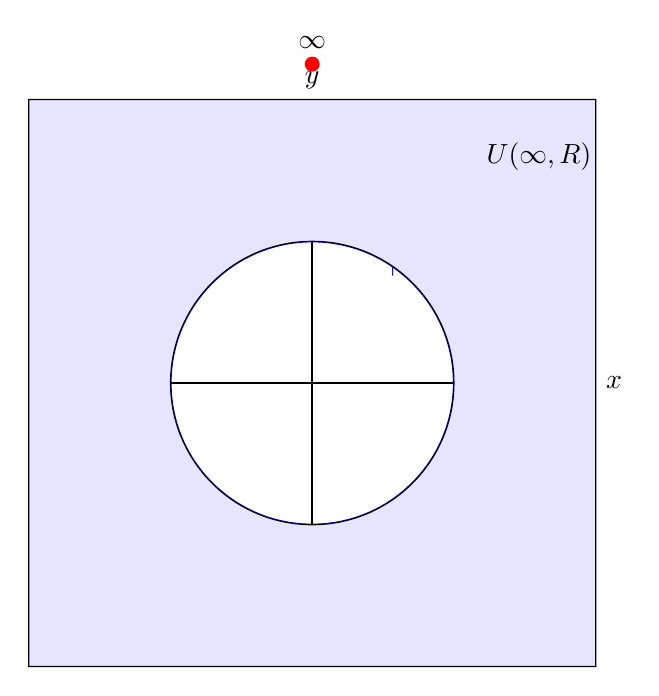
\begin{tikzpicture}[scale=0.9]
    % 坐标轴
    \draw[->, thick] (-4, 0) -- (4, 0) node[right] {$x$};
    \draw[->, thick] (0, -4) -- (0, 4) node[above] {$y$};
    
    % 圆
    \draw[blue, thick] (0, 0) circle (2);
    \node[blue] at (1.7, 1.7) {$|z| = R$};
    
    % 外部区域（阴影）
    \draw[fill=blue!10, even odd rule] (-4, -4) rectangle (4, 4) (0, 0) circle (2);
    
    % 无穷远点
    \node at (0, 4.8) {$\infty$};
    \fill[red] (0, 4.5) circle (3pt);
    
    % 标注
    \node at (3.2, 3.2) {$U(\infty, R)$};
\end{tikzpicture}
\caption{无穷远点的邻域：圆外区域}
\label{fig:infinity-neighborhood}
\end{figure}

\begin{wulibj}[复球面的好处]
复球面提供了一个完美的拓扑图景：
\begin{enumerate}
    \item \textbf{紧致性}：$\overline{\mathbb{C}}$ 是紧致的（类似于闭区间 $[a, b]$），而 $\mathbb{C}$ 不是。这意味着在 $\overline{\mathbb{C}}$ 上，任何无穷点列都有收敛子列。
    \item \textbf{统一性}：无穷远点和有限点地位平等，都是球面上的普通点。
    \item \textbf{留数理论}：我们可以定义无穷远点的留数，使留数定理更完整。
    \item \textbf{保角映射}：奇点的分类和讨论更方便。
\end{enumerate}
\end{wulibj}

\begin{lizi}{}{}
在扩充复平面上，圆 $|z| = 1$ 把平面分成两部分：内部和外部。问这两部分在复球面上分别是什么形状？
 \begin{jie}
    在复球面上：
    \begin{itemize}
        \item 圆的内部 $|z| < 1$ 映射为球面上靠近南极的球冠。
        \item 圆的外部 $|z| > 1$（连同 $\infty$）映射为球面上靠近北极的球冠。
        \item 圆周 $|z| = 1$ 映射为球面上的纬线圈。
    \end{itemize}
    所以，一个圆把球面分成两个球冠，地位是平等的。
 \end{jie}
\end{lizi}

\subsection{复球面上的直线与圆}

在复球面上，直线和圆有统一的观点。

\begin{dingli}{}{扩充复平面上的圆}
在扩充复平面上，\textbf{圆}是满足方程
\begin{equation}
    A|z|^2 + \bar{B}z + B\bar{z} + C = 0
\end{equation}
的点集，其中 $A, C \in \mathbb{R}$，$B \in \mathbb{C}$，且 $|B|^2 > AC$（保证曲线非退化）。

特别地：
\begin{itemize}
    \item 当 $A \neq 0$ 时，是普通圆（圆心 $-B/A$，半径 $\sqrt{|B|^2 - AC}/|A|$）。
    \item 当 $A = 0$ 时，是直线（过无穷远点）。
\end{itemize}
\end{dingli}

这个统一观点在研究保角映射时非常有用——保角映射把圆变成圆（广义的，包括直线）。

% ========== 第六节 ==========
\section{复数\index{复数}的应用：交流电路、量子力学}

前面我们学习了复数\index{复数}的基本概念和运算。现在让我们看看复数\index{复数}在物理中的两个重要应用。

\subsection{交流电路中的复数\index{复数}方法}

在交流电路中，电压和电流都是时间的正弦函数。直接用三角函数进行运算非常繁琐，而用复数\index{复数}表示则可以大大简化计算。

\subsubsection{相量表示}

设电压和电流为
\begin{align}
    u(t) &= U_0 \cos(\omega t + \varphi_u) \\
    i(t) &= I_0 \cos(\omega t + \varphi_i)
\end{align}
其中 $U_0$、$I_0$ 是振幅，$\omega$ 是角频率，$\varphi_u$、$\varphi_i$ 是初相位。

引入\textbf{相量}（复数\index{复数}）表示：
\begin{align}
    \dot{U} &= U_0 \mathrm{e}^{\mathrm{i}\varphi_u} \\
    \dot{I} &= I_0 \mathrm{e}^{\mathrm{i}\varphi_i}
\end{align}

注意：相量只包含振幅和相位信息，不包含频率。同一频率的交流量才能用相量运算。

\subsubsection{阻抗的复数\index{复数}表示}

对于电阻 $R$、电感 $L$、电容 $C$，定义\textbf{复阻抗}：
\begin{align}
    Z_R &= R \\
    Z_L &= \mathrm{i}\omega L \\
    Z_C &= \frac{1}{\mathrm{i}\omega C} = -\frac{\mathrm{i}}{\omega C}
\end{align}

\begin{tishi}[为什么电感阻抗有 $\mathrm{i}$？]
电感两端的电压 $u = L \frac{\mathrm{d}i}{\mathrm{d}t}$。若 $i = I_0 \cos(\omega t)$，则
\begin{equation}
    u = -L\omega I_0 \sin(\omega t) = L\omega I_0 \cos\left(\omega t + \frac{\pi}{2}\right)
\end{equation}
电压超前电流 $\pi/2$，即 $90°$。这正是 $\mathrm{i} = \mathrm{e}^{\mathrm{i}\pi/2}$ 的效果。
\end{tishi}

\subsubsection{欧姆定律的复数\index{复数}形式}

复数\index{复数}形式的欧姆定律为
\begin{equation}
    \dot{U} = Z \dot{I}
\end{equation}

这与直流电路的欧姆定律形式完全相同！

\begin{lizi}{}{}
电阻 $R = 30\,\Omega$ 与电感 $L = 40\,\mathrm{mH}$ 串联，电源 $u(t) = 220\sqrt{2}\cos(100\pi t)\,\mathrm{V}$。\\求电流的有效值与初相位。

\begin{jie}
    角频率 $\omega = 100\pi\,\mathrm{rad/s}$。
    
    复阻抗为
    \begin{equation}
        Z = R + \mathrm{i}\omega L = 30 + \mathrm{i} \cdot 100\pi \cdot 0.04 = 30 + \mathrm{i} \cdot 4\pi \approx 30 + \mathrm{i} \cdot 12.57\,\Omega
    \end{equation}
    
    阻抗的模为
    \begin{equation}
        |Z| = \sqrt{30^2 + 12.57^2} \approx 32.5\,\Omega
    \end{equation}
    
    电压有效值 $U = 220\,\mathrm{V}$，所以电流有效值为
    \begin{equation}
        I = \frac{U}{|Z|} = \frac{220}{32.5} \approx 6.77\,\mathrm{A}
    \end{equation}
    
    电流滞后电压的相位角为
    \begin{equation}
        \varphi = \arctan\frac{\omega L}{R} = \arctan\frac{12.57}{30} \approx 22.7°
    \end{equation}
\end{jie}
\end{lizi}

\subsection{量子力学中的复数\index{复数}}

在量子力学中，\textbf{波函数} $\psi(x, t)$ 是一个复值函数，其物理意义由玻恩给出：

\begin{dingliyi}{}{玻恩统计诠释}
波函数的模方 $|\psi(x, t)|^2 = \psi^*(x, t) \psi(x, t)$ 表示在时刻 $t$、位置 $x$ 处找到粒子的概率密度。
\end{dingliyi}

这里 $\psi^*$ 表示 $\psi$ 的复共轭。

\begin{wulibj}[为什么量子力学需要复数？]
在经典物理中，我们用实数描述物理量。但在量子力学中，复数\index{复数}是必不可少的：

\begin{enumerate}
    \item \textbf{干涉现象}：量子叠加原理要求波函数有相位。两个波函数叠加时，干涉项 $\psi_1^* \psi_2$ 依赖于相对相位，这需要复数\index{复数}。

    \item \textbf{时间演化}：薛定谔方程 $\mathrm{i}\hbar \frac{\partial \psi}{\partial t} = \hat{H}\psi$ 中有虚数单位 $\mathrm{i}$。这保证了概率守恒。

    \item \textbf{可观测量}：虽然波函数是复数\index{复数}，但可观测量（如概率密度、能量、动量）都是实数，由厄米算符的本征值给出。
\end{enumerate}
\end{wulibj}

\begin{lizi}{}{}
自由粒子的波函数为
\begin{equation}
    \psi(x, t) = A \mathrm{e}^{\mathrm{i}(kx - \omega t)}
\end{equation}
其中 $A$ 是归一化常数，$k = p/\hbar$ 是波数，$\omega = E/\hbar$ 是角频率。

验证：概率密度 $|\psi|^2$ 与时间和位置无关。

\begin{jie}
    复共轭为
    \begin{equation}
        \psi^* = A^* \mathrm{e}^{-\mathrm{i}(kx - \omega t)}
    \end{equation}
    
    概率密度为
    \begin{equation}
        |\psi|^2 = \psi^* \psi = |A|^2 \mathrm{e}^{-\mathrm{i}(kx - \omega t)} \mathrm{e}^{\mathrm{i}(kx - \omega t)} = |A|^2
    \end{equation}
    
    这确实是一个常数，说明自由粒子在各处出现的概率相等。
\end{jie}
\end{lizi}

% ========== 本章小结 ==========
\section{本章小结}

\subsection{知识框架}

本章我们建立了复数\index{复数}的基本理论框架：

\begin{center}
\begin{tikzpicture}[node distance=1.2cm, auto,
    % 定义框样式（绿色）
    defblock/.style={rectangle, draw=defteal, fill=defteal!15, text width=5.5em, text centered, rounded corners, minimum height=2em, font=\small, line width=0.8pt},
    % 概念框样式（蓝色）
    conblock/.style={rectangle, draw=theoremblue, fill=theoremblue!15, text width=5.5em, text centered, rounded corners, minimum height=2em, font=\small, line width=0.8pt},
    % 运算框样式（紫色）
    opblock/.style={rectangle, draw=examplepurple, fill=examplepurple!15, text width=5.5em, text centered, rounded corners, minimum height=2em, font=\small, line width=0.8pt},
    line/.style={draw, -latex, thick, gray!70}]
    
    % 第一层
    \node[defblock] (def) {复数定义 $z=x+\mathrm{i}y$};
    \node[conblock, right=of def] (geom) {几何表示\\复平面};
    \node[conblock, right=of geom] (form) {三种形式\\代数/三角/指数};
    \node[conblock, right=of form] (sphere) {复球面\\无穷远点};
    
    % 第二层
    \node[conblock, below=of def] (mod) {模 $|z|$};
    \node[conblock, below=of geom] (arg) {辐角 $\theta$};
    \node[conblock, below=of form] (conj) {共轭 $\bar{z}$};
    \node[conblock, below=of sphere] (extend) {扩充复平面\\ $\overline{\mathbb{C}}$};
    
    % 第三层
    \node[opblock, below=1.2cm of mod, xshift=2cm] (op) {运算\\四则/幂/根};
    \node[opblock, below=1.2cm of arg, xshift=2cm] (set) {点集\\区域/连通性};
    
    \path[line] (def) -- (geom);
    \path[line] (geom) -- (form);
    \path[line] (form) -- (sphere);
    \path[line] (geom) -- (mod);
    \path[line] (geom) -- (arg);
    \path[line] (form) -- (conj);
    \path[line] (sphere) -- (extend);
    \path[line] (mod) -- (op);
    \path[line] (arg) -- (op);
    \path[line] (conj) -- (op);
    \path[line] (geom) -- (set);
\end{tikzpicture}
\end{center}

\subsection{核心公式}

\begin{table}[htbp]
\centering
\begin{tabular}{ll}
\toprule
\textbf{内容} & \textbf{公式/概念} \\
\midrule
复数\index{复数}定义 & $z = x + \mathrm{i}y$ \\
模 & $|z| = \sqrt{x^2 + y^2}$ \\
辐角 & $\tan\theta = y/x$ \\
三角形式 & $z = r(\cos\theta + \mathrm{i}\sin\theta)$ \\
指数形式 & $z = r\mathrm{e}^{\mathrm{i}\theta}$ \\
共轭 & $\bar{z} = x - \mathrm{i}y$ \\
乘法（指数形式） & $z_1 z_2 = r_1 r_2 \mathrm{e}^{\mathrm{i}(\theta_1 + \theta_2)}$ \\
棣莫弗公式 & $(\cos\theta + \mathrm{i}\sin\theta)^n = \cos n\theta + \mathrm{i}\sin n\theta$ \\
$n$ 次方根 & $w_k = \sqrt[n]{r} \, \mathrm{e}^{\mathrm{i}(\theta + 2k\pi)/n}$ \\
\midrule
扩充复平面 & $\overline{\mathbb{C}} = \mathbb{C} \cup \{\infty\}$ \\
球极投影 & 复平面 $\longleftrightarrow$ 复球面（北极对应 $\infty$） \\
\bottomrule
\end{tabular}
\caption{本章核心公式与概念}
\label{tab:formulas-ch1}
\end{table}

\subsection{易错点提醒}

\begin{enumerate}
    \item \textbf{虚部的定义}：虚部是 $y$，不是 $\mathrm{i}y$。
    \item \textbf{辐角计算}：不能用 $\theta = \arctan(y/x)$ 直接计算，需要考虑象限。
    \item \textbf{开方多值性}：$n$ 次方根有 $n$ 个值，不要遗漏。
    \item \textbf{区域连通性}：单连通区域``没有洞''，多连通区域``有洞''，这对后续积分定理很重要。
    \item \textbf{无穷远点的唯一性}：复平面中只有一个无穷远点 $\infty$，不像实数有 $+\infty$ 和 $-\infty$ 之分。
    \item \textbf{不定式}：$\infty - \infty$、$\infty \cdot 0$、$\frac{\infty}{\infty}$、$\frac{0}{0}$ 都无定义，需要具体情况具体分析。
\end{enumerate}

% ========== 习题 ==========
\section{习题}

\textbf{基础题}

\begin{enumerate}
    \item 计算下列复数\index{复数}的模和主辐角：
    \begin{enumerate}
        \item $z = 1 + \mathrm{i}$
        \item $z = -1 + \sqrt{3}\mathrm{i}$
        \item $z = -2 - 2\mathrm{i}$
        \item $z = 3 - 4\mathrm{i}$
    \end{enumerate}
    
    \item 将下列复数\index{复数}化为指数形式：
    \begin{enumerate}
        \item $z = 1 - \mathrm{i}$
        \item $z = -\sqrt{3} + \mathrm{i}$
        \item $z = 2 + 2\sqrt{3}\mathrm{i}$
    \end{enumerate}
    
    \item 计算：
    \begin{enumerate}
        \item $(1 + \mathrm{i})^8$
        \item $\displaystyle\frac{1 + \mathrm{i}}{1 - \mathrm{i}}$
        \item $\sqrt[3]{-8}$
    \end{enumerate}
    
    \item 求 $z^4 + 1 = 0$ 的所有根。
\end{enumerate}

\textbf{综合题}

\begin{enumerate}[resume]
    \item 设 $z_1 = r_1 \mathrm{e}^{\mathrm{i}\theta_1}$，$z_2 = r_2 \mathrm{e}^{\mathrm{i}\theta_2}$，证明：
    \begin{enumerate}
        \item $|z_1 z_2| = |z_1| \cdot |z_2|$
        \item $\left|\frac{z_1}{z_2}\right| = \frac{|z_1|}{|z_2|}$（$z_2 \neq 0$）
    \end{enumerate}
    
    \item 利用棣莫弗公式证明：
    \begin{enumerate}
        \item $\sin 3\theta = 3\sin\theta - 4\sin^3\theta$
        \item $\cos 4\theta = 8\cos^4\theta - 8\cos^2\theta + 1$
    \end{enumerate}
    
    \item 设 $z \neq 0$，证明：
    \begin{equation}
        \operatorname{Re}(z) = \frac{z + \bar{z}}{2}, \quad \operatorname{Im}(z) = \frac{z - \bar{z}}{2\mathrm{i}}
    \end{equation}
    
    \item 证明：$|z_1 + z_2| \leq |z_1| + |z_2|$（三角不等式），并说明几何意义。
\end{enumerate}

\textbf{挑战题}

\begin{enumerate}[resume]
    \item 设 $z_1, z_2, z_3$ 是复平面上三角形的三个顶点，证明：
    \begin{enumerate}
        \item 三角形的重心为 $\displaystyle\frac{z_1 + z_2 + z_3}{3}$
        \item 若 $|z_1| = |z_2| = |z_3|$，则三角形的外心在原点
    \end{enumerate}
    
    \item 设 $z = x + \mathrm{i}y$，证明：
    \begin{equation}
        \mathrm{e}^z = \mathrm{e}^x(\cos y + \mathrm{i}\sin y)
    \end{equation}
    由此说明 $\mathrm{e}^z$ 的周期性。
    
    \item 在复平面上描绘下列点集：
    \begin{enumerate}
        \item $\{z : |z - 1| < 2\}$
        \item $\{z : |z - 1| = |z + 1|\}$
        \item $\{z : 1 < |z| < 2\}$
        \item $\{z : \operatorname{Re}(z) > 0, |z| < 1\}$
    \end{enumerate}
    并判断每个集合是否为区域，是单连通还是多连通。
\end{enumerate}
